\documentclass[1p]{elsarticle_modified}
%\bibliographystyle{elsarticle-num}

%\usepackage[colorlinks]{hyperref}
%\usepackage{abbrmath_seonhwa} %\Abb, \Ascr, \Acal ,\Abf, \Afrak
\usepackage{amsfonts}
\usepackage{amssymb}
\usepackage{amsmath}
\usepackage{amsthm}
\usepackage{scalefnt}
\usepackage{amsbsy}
\usepackage{kotex}
\usepackage{caption}
\usepackage{subfig}
\usepackage{color}
\usepackage{graphicx}
\usepackage{xcolor} %% white, black, red, green, blue, cyan, magenta, yellow
\usepackage{float}
\usepackage{setspace}
\usepackage{hyperref}

\usepackage{tikz}
\usetikzlibrary{arrows}

\usepackage{multirow}
\usepackage{array} % fixed length table
\usepackage{hhline}

%%%%%%%%%%%%%%%%%%%%%
\makeatletter
\renewcommand*\env@matrix[1][\arraystretch]{%
	\edef\arraystretch{#1}%
	\hskip -\arraycolsep
	\let\@ifnextchar\new@ifnextchar
	\array{*\c@MaxMatrixCols c}}
\makeatother %https://tex.stackexchange.com/questions/14071/how-can-i-increase-the-line-spacing-in-a-matrix
%%%%%%%%%%%%%%%

\usepackage[normalem]{ulem}

\newcommand{\msout}[1]{\ifmmode\text{\sout{\ensuremath{#1}}}\else\sout{#1}\fi}
%SOURCE: \msout is \stkout macro in https://tex.stackexchange.com/questions/20609/strikeout-in-math-mode

\newcommand{\cancel}[1]{
	\ifmmode
	{\color{red}\msout{#1}}
	\else
	{\color{red}\sout{#1}}
	\fi
}

\newcommand{\add}[1]{
	{\color{blue}\uwave{#1}}
}

\newcommand{\replace}[2]{
	\ifmmode
	{\color{red}\msout{#1}}{\color{blue}\uwave{#2}}
	\else
	{\color{red}\sout{#1}}{\color{blue}\uwave{#2}}
	\fi
}

\newcommand{\Sol}{\mathcal{S}} %segment
\newcommand{\D}{D} %diagram
\newcommand{\A}{\mathcal{A}} %arc


%%%%%%%%%%%%%%%%%%%%%%%%%%%%%5 test

\def\sl{\operatorname{\textup{SL}}(2,\Cbb)}
\def\psl{\operatorname{\textup{PSL}}(2,\Cbb)}
\def\quan{\mkern 1mu \triangleright \mkern 1mu}

\theoremstyle{definition}
\newtheorem{thm}{Theorem}[section]
\newtheorem{prop}[thm]{Proposition}
\newtheorem{lem}[thm]{Lemma}
\newtheorem{ques}[thm]{Question}
\newtheorem{cor}[thm]{Corollary}
\newtheorem{defn}[thm]{Definition}
\newtheorem{exam}[thm]{Example}
\newtheorem{rmk}[thm]{Remark}
\newtheorem{alg}[thm]{Algorithm}

\newcommand{\I}{\sqrt{-1}}
\begin{document}

%\begin{frontmatter}
%
%\title{Boundary parabolic representations of knots up to 8 crossings}
%
%%% Group authors per affiliation:
%\author{Yunhi Cho} 
%\address{Department of Mathematics, University of Seoul, Seoul, Korea}
%\ead{yhcho@uos.ac.kr}
%
%
%\author{Seonhwa Kim} %\fnref{s_kim}}
%\address{Center for Geometry and Physics, Institute for Basic Science, Pohang, 37673, Korea}
%\ead{ryeona17@ibs.re.kr}
%
%\author{Hyuk Kim}
%\address{Department of Mathematical Sciences, Seoul National University, Seoul 08826, Korea}
%\ead{hyukkim@snu.ac.kr}
%
%\author{Seokbeom Yoon}
%\address{Department of Mathematical Sciences, Seoul National University, Seoul, 08826,  Korea}
%\ead{sbyoon15@snu.ac.kr}
%
%\begin{abstract}
%We find all boundary parabolic representation of knots up to 8 crossings.
%
%\end{abstract}
%\begin{keyword}
%    \MSC[2010] 57M25 
%\end{keyword}
%
%\end{frontmatter}

%\linenumbers
%\tableofcontents
%
\newcommand\colored[1]{\textcolor{white}{\rule[-0.35ex]{0.8em}{1.4ex}}\kern-0.8em\color{red} #1}%
%\newcommand\colored[1]{\textcolor{white}{ #1}\kern-2.17ex	\textcolor{white}{ #1}\kern-1.81ex	\textcolor{white}{ #1}\kern-2.15ex\color{red}#1	}

{\Large $\underline{12a_{0184}~(K12a_{0184})}$}

\setlength{\tabcolsep}{10pt}
\renewcommand{\arraystretch}{1.6}
\vspace{1cm}\begin{tabular}{m{100pt}>{\centering\arraybackslash}m{274pt}}
\multirow{5}{120pt}{
	\centering
	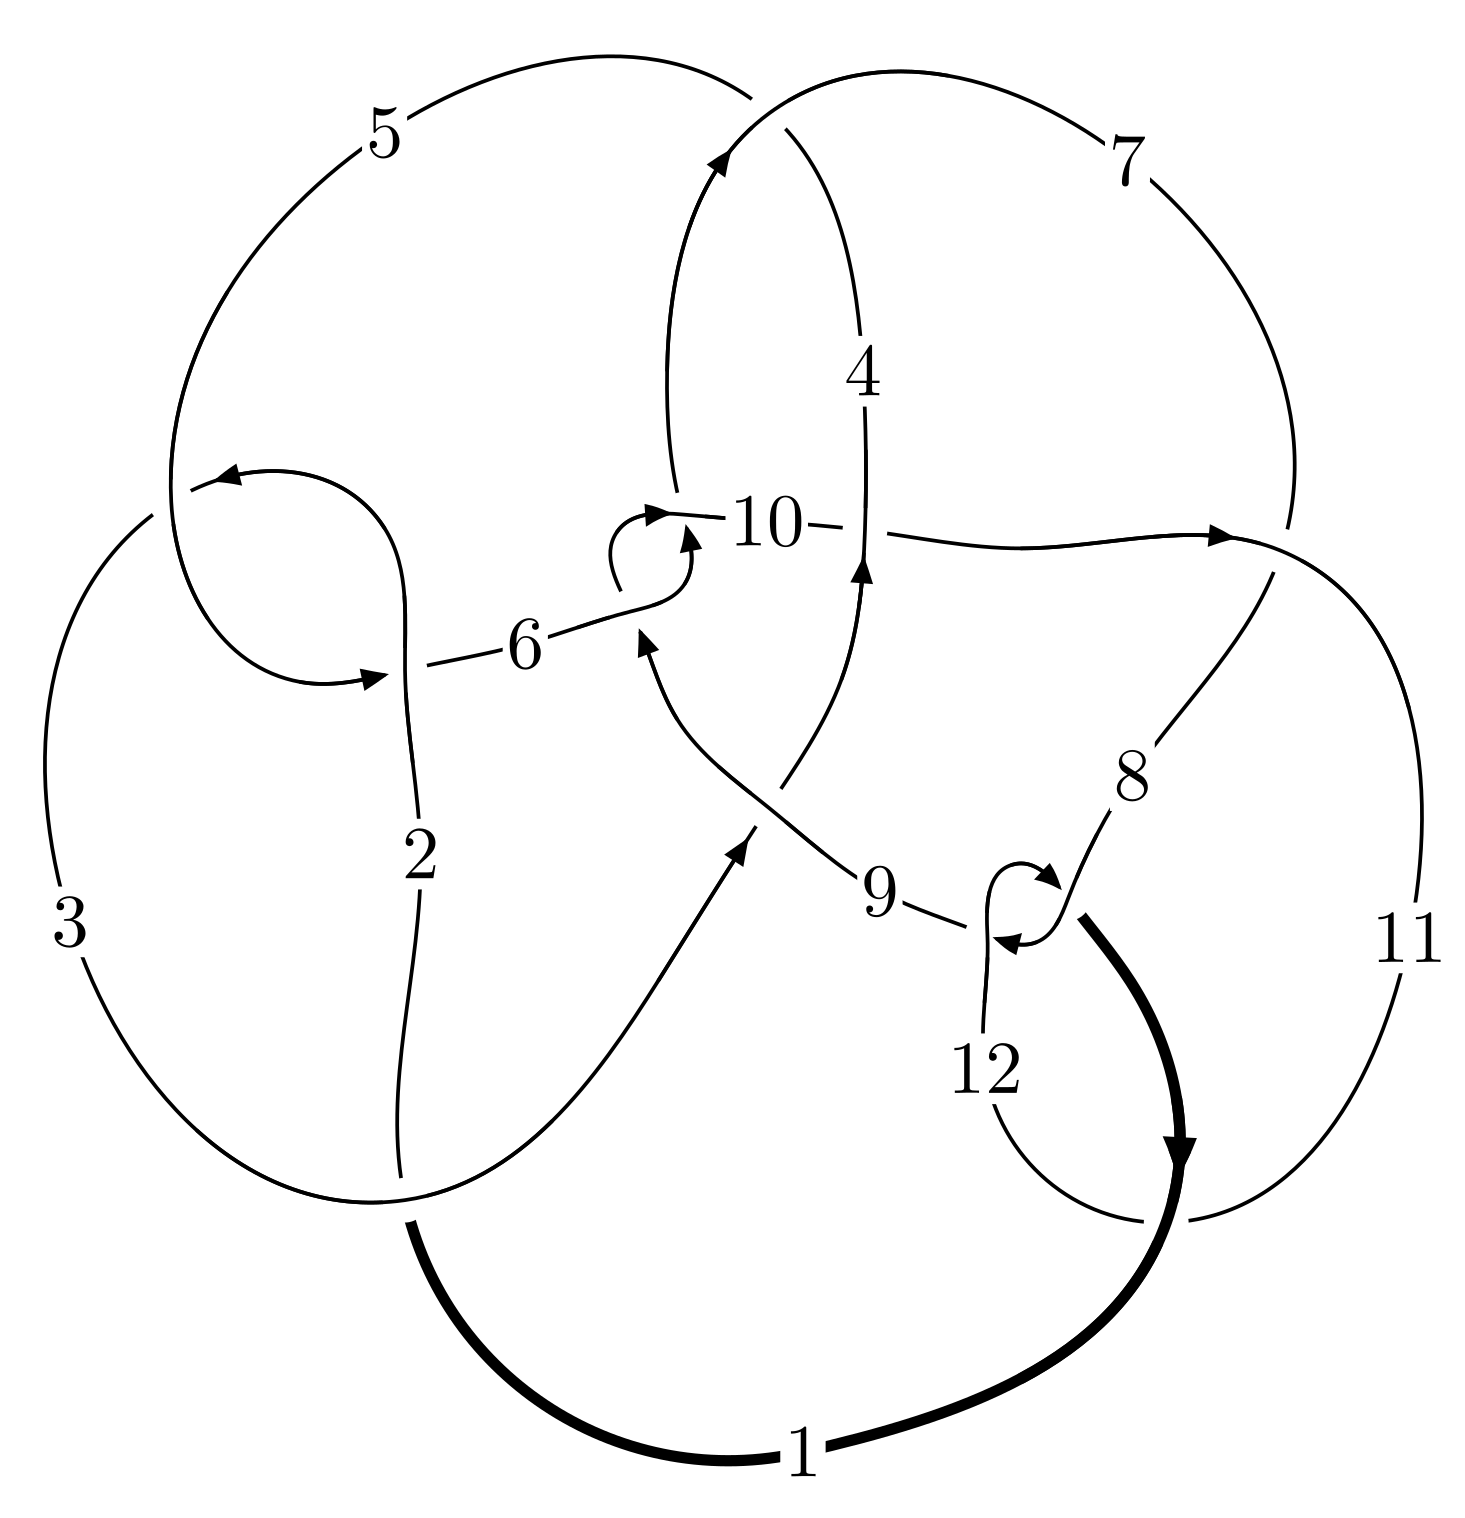
\includegraphics[width=112pt]{../../../GIT/diagram.site/Diagrams/png/985_12a_0184.png}\\
\ \ \ A knot diagram\footnotemark}&
\allowdisplaybreaks
\textbf{Linearized knot diagam} \\
\cline{2-2}
 &
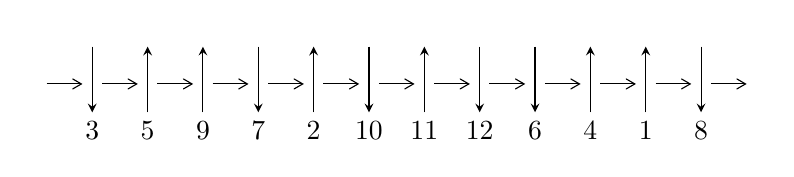
\begin{tikzpicture}[x=20pt, y=17pt]
	% nodes
	\node (C0) at (0, 0) {};
	\node (C1) at (1, 0) {};
	\node (C1U) at (1, +1) {};
	\node (C1D) at (1, -1) {3};

	\node (C2) at (2, 0) {};
	\node (C2U) at (2, +1) {};
	\node (C2D) at (2, -1) {5};

	\node (C3) at (3, 0) {};
	\node (C3U) at (3, +1) {};
	\node (C3D) at (3, -1) {9};

	\node (C4) at (4, 0) {};
	\node (C4U) at (4, +1) {};
	\node (C4D) at (4, -1) {7};

	\node (C5) at (5, 0) {};
	\node (C5U) at (5, +1) {};
	\node (C5D) at (5, -1) {2};

	\node (C6) at (6, 0) {};
	\node (C6U) at (6, +1) {};
	\node (C6D) at (6, -1) {10};

	\node (C7) at (7, 0) {};
	\node (C7U) at (7, +1) {};
	\node (C7D) at (7, -1) {11};

	\node (C8) at (8, 0) {};
	\node (C8U) at (8, +1) {};
	\node (C8D) at (8, -1) {12};

	\node (C9) at (9, 0) {};
	\node (C9U) at (9, +1) {};
	\node (C9D) at (9, -1) {6};

	\node (C10) at (10, 0) {};
	\node (C10U) at (10, +1) {};
	\node (C10D) at (10, -1) {4};

	\node (C11) at (11, 0) {};
	\node (C11U) at (11, +1) {};
	\node (C11D) at (11, -1) {1};

	\node (C12) at (12, 0) {};
	\node (C12U) at (12, +1) {};
	\node (C12D) at (12, -1) {8};
	\node (C13) at (13, 0) {};

	% arrows
	\draw[->,>={angle 60}]
	(C0) edge (C1) (C1) edge (C2) (C2) edge (C3) (C3) edge (C4) (C4) edge (C5) (C5) edge (C6) (C6) edge (C7) (C7) edge (C8) (C8) edge (C9) (C9) edge (C10) (C10) edge (C11) (C11) edge (C12) (C12) edge (C13) ;	\draw[->,>=stealth]
	(C1U) edge (C1D) (C2D) edge (C2U) (C3D) edge (C3U) (C4U) edge (C4D) (C5D) edge (C5U) (C6U) edge (C6D) (C7D) edge (C7U) (C8U) edge (C8D) (C9U) edge (C9D) (C10D) edge (C10U) (C11D) edge (C11U) (C12U) edge (C12D) ;
	\end{tikzpicture} \\
\hhline{~~} \\& 
\textbf{Solving Sequence} \\ \cline{2-2} 
 &
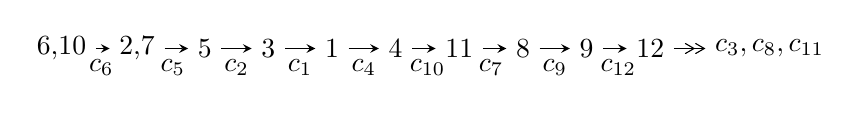
\begin{tikzpicture}[x=23pt, y=7pt]
	% node
	\node (A0) at (-1/8, 0) {6,10};
	\node (A1) at (17/16, 0) {2,7};
	\node (A2) at (17/8, 0) {5};
	\node (A3) at (25/8, 0) {3};
	\node (A4) at (33/8, 0) {1};
	\node (A5) at (41/8, 0) {4};
	\node (A6) at (49/8, 0) {11};
	\node (A7) at (57/8, 0) {8};
	\node (A8) at (65/8, 0) {9};
	\node (A9) at (73/8, 0) {12};
	\node (C1) at (1/2, -1) {$c_{6}$};
	\node (C2) at (13/8, -1) {$c_{5}$};
	\node (C3) at (21/8, -1) {$c_{2}$};
	\node (C4) at (29/8, -1) {$c_{1}$};
	\node (C5) at (37/8, -1) {$c_{4}$};
	\node (C6) at (45/8, -1) {$c_{10}$};
	\node (C7) at (53/8, -1) {$c_{7}$};
	\node (C8) at (61/8, -1) {$c_{9}$};
	\node (C9) at (69/8, -1) {$c_{12}$};
	\node (A10) at (11, 0) {$c_{3},c_{8},c_{11}$};

	% edge
	\draw[->,>=stealth]	
	(A0) edge (A1) (A1) edge (A2) (A2) edge (A3) (A3) edge (A4) (A4) edge (A5) (A5) edge (A6) (A6) edge (A7) (A7) edge (A8) (A8) edge (A9) ;
	\draw[->>,>={angle 60}]	
	(A9) edge (A10);
\end{tikzpicture} \\ 

\end{tabular} \\

\footnotetext{
The image of knot diagram is generated by the software ``\textbf{Draw programme}" developed by Andrew Bartholomew(\url{http://www.layer8.co.uk/maths/draw/index.htm\#Running-draw}), where we modified some parts for our purpose(\url{https://github.com/CATsTAILs/LinksPainter}).
}\phantom \\ \newline 
\centering \textbf{Ideals for irreducible components\footnotemark of $X_{\text{par}}$} 
 
\begin{align*}
I^u_{1}&=\langle 
1.32502\times10^{415} u^{119}+2.54170\times10^{414} u^{118}+\cdots+4.01044\times10^{414} b+1.64747\times10^{415},\\
\phantom{I^u_{1}}&\phantom{= \langle  }-2.94399\times10^{415} u^{119}+8.35823\times10^{413} u^{118}+\cdots+4.01044\times10^{414} a-4.49947\times10^{415},\\
\phantom{I^u_{1}}&\phantom{= \langle  }u^{120}+u^{119}+\cdots+10 u^3+1\rangle \\
\\
\end{align*}
\raggedright * 1 irreducible components of $\dim_{\mathbb{C}}=0$, with total 120 representations.\\
\footnotetext{All coefficients of polynomials are rational numbers. But the coefficients are sometimes approximated in decimal forms when there is not enough margin.}
\newpage
\renewcommand{\arraystretch}{1}
\centering \section*{I. $I^u_{1}= \langle 1.33\times10^{415} u^{119}+2.54\times10^{414} u^{118}+\cdots+4.01\times10^{414} b+1.65\times10^{415},\;-2.94\times10^{415} u^{119}+8.36\times10^{413} u^{118}+\cdots+4.01\times10^{414} a-4.50\times10^{415},\;u^{120}+u^{119}+\cdots+10 u^3+1 \rangle$}
\flushleft \textbf{(i) Arc colorings}\\
\begin{tabular}{m{7pt} m{180pt} m{7pt} m{180pt} }
\flushright $a_{6}=$&$\begin{pmatrix}1\\0\end{pmatrix}$ \\
\flushright $a_{10}=$&$\begin{pmatrix}0\\u\end{pmatrix}$ \\
\flushright $a_{2}=$&$\begin{pmatrix}7.34081 u^{119}-0.208412 u^{118}+\cdots-10.6447 u+11.2194\\-3.30393 u^{119}-0.633771 u^{118}+\cdots+6.62963 u-4.10796\end{pmatrix}$ \\
\flushright $a_{7}=$&$\begin{pmatrix}1\\u^2\end{pmatrix}$ \\
\flushright $a_{5}=$&$\begin{pmatrix}4.01710 u^{119}+0.119879 u^{118}+\cdots-3.90539 u+6.04797\\-3.21398 u^{119}-0.625442 u^{118}+\cdots+6.57033 u-4.99074\end{pmatrix}$ \\
\flushright $a_{3}=$&$\begin{pmatrix}1.45823 u^{119}-0.337341 u^{118}+\cdots+1.35147 u+1.99223\\-3.87235 u^{119}-0.835695 u^{118}+\cdots+7.67638 u-6.04582\end{pmatrix}$ \\
\flushright $a_{1}=$&$\begin{pmatrix}-0.465417 u^{119}-0.193298 u^{118}+\cdots+0.190894 u-1.89568\\-1.79434 u^{119}-0.567792 u^{118}+\cdots+3.10178 u-2.81939\end{pmatrix}$ \\
\flushright $a_{4}=$&$\begin{pmatrix}-2.41952 u^{119}-0.429440 u^{118}+\cdots+6.68204 u-2.83999\\-7.75010 u^{119}-0.927794 u^{118}+\cdots+13.0070 u-10.8780\end{pmatrix}$ \\
\flushright $a_{11}=$&$\begin{pmatrix}2.81939 u^{119}+1.02505 u^{118}+\cdots-7.07901 u+3.10178\\0.272120 u^{119}+0.227342 u^{118}+\cdots-1.89568 u+0.465417\end{pmatrix}$ \\
\flushright $a_{8}=$&$\begin{pmatrix}-0.449390 u^{119}-0.0914268 u^{118}+\cdots+0.730282 u+0.133441\\0.589239 u^{119}-0.181546 u^{118}+\cdots-0.203075 u+0.449511\end{pmatrix}$ \\
\flushright $a_{9}=$&$\begin{pmatrix}u\\u\end{pmatrix}$ \\
\flushright $a_{12}=$&$\begin{pmatrix}1.84197 u^{119}+0.631727 u^{118}+\cdots-6.73022 u+2.27079\\1.07750 u^{119}+0.405949 u^{118}+\cdots-2.93100 u+1.45822\end{pmatrix}$\\&\end{tabular}
\flushleft \textbf{(ii) Obstruction class $= -1$}\\~\\
\flushleft \textbf{(iii) Cusp Shapes $= 64.8920 u^{119}+14.0763 u^{118}+\cdots-80.1155 u+70.0515$}\\~\\
\newpage\renewcommand{\arraystretch}{1}
\flushleft \textbf{(iv) u-Polynomials at the component}\newline \\
\begin{tabular}{m{50pt}|m{274pt}}
Crossings & \hspace{64pt}u-Polynomials at each crossing \\
\hline $$\begin{aligned}c_{1}\end{aligned}$$&$\begin{aligned}
&u^{120}+49 u^{119}+\cdots+140 u+1
\end{aligned}$\\
\hline $$\begin{aligned}c_{2},c_{5}\end{aligned}$$&$\begin{aligned}
&u^{120}+u^{119}+\cdots+20 u+1
\end{aligned}$\\
\hline $$\begin{aligned}c_{3}\end{aligned}$$&$\begin{aligned}
&u^{120}-15 u^{119}+\cdots-620400 u+166375
\end{aligned}$\\
\hline $$\begin{aligned}c_{4}\end{aligned}$$&$\begin{aligned}
&u^{120}+5 u^{119}+\cdots-14 u+1
\end{aligned}$\\
\hline $$\begin{aligned}c_{6},c_{9}\end{aligned}$$&$\begin{aligned}
&u^{120}+u^{119}+\cdots+10 u^3+1
\end{aligned}$\\
\hline $$\begin{aligned}c_{7}\end{aligned}$$&$\begin{aligned}
&u^{120}-5 u^{119}+\cdots-1412636 u+186749
\end{aligned}$\\
\hline $$\begin{aligned}c_{8},c_{12}\end{aligned}$$&$\begin{aligned}
&u^{120}+5 u^{119}+\cdots+2 u+1
\end{aligned}$\\
\hline $$\begin{aligned}c_{10}\end{aligned}$$&$\begin{aligned}
&u^{120}-3 u^{119}+\cdots-4 u+1
\end{aligned}$\\
\hline $$\begin{aligned}c_{11}\end{aligned}$$&$\begin{aligned}
&u^{120}-61 u^{119}+\cdots-10 u^2+1
\end{aligned}$\\
\hline
\end{tabular}\\~\\
\newpage\renewcommand{\arraystretch}{1}
\flushleft \textbf{(v) Riley Polynomials at the component}\newline \\
\begin{tabular}{m{50pt}|m{274pt}}
Crossings & \hspace{64pt}Riley Polynomials at each crossing \\
\hline $$\begin{aligned}c_{1}\end{aligned}$$&$\begin{aligned}
&y^{120}+45 y^{119}+\cdots+3100 y+1
\end{aligned}$\\
\hline $$\begin{aligned}c_{2},c_{5}\end{aligned}$$&$\begin{aligned}
&y^{120}+49 y^{119}+\cdots+140 y+1
\end{aligned}$\\
\hline $$\begin{aligned}c_{3}\end{aligned}$$&$\begin{aligned}
&y^{120}-71 y^{119}+\cdots-1592489167500 y+27680640625
\end{aligned}$\\
\hline $$\begin{aligned}c_{4}\end{aligned}$$&$\begin{aligned}
&y^{120}-87 y^{119}+\cdots+408 y+1
\end{aligned}$\\
\hline $$\begin{aligned}c_{6},c_{9}\end{aligned}$$&$\begin{aligned}
&y^{120}-75 y^{119}+\cdots-50 y^2+1
\end{aligned}$\\
\hline $$\begin{aligned}c_{7}\end{aligned}$$&$\begin{aligned}
&y^{120}-67 y^{119}+\cdots+1230496216784 y+34875189001
\end{aligned}$\\
\hline $$\begin{aligned}c_{8},c_{12}\end{aligned}$$&$\begin{aligned}
&y^{120}+61 y^{119}+\cdots-10 y^2+1
\end{aligned}$\\
\hline $$\begin{aligned}c_{10}\end{aligned}$$&$\begin{aligned}
&y^{120}+5 y^{119}+\cdots-12 y+1
\end{aligned}$\\
\hline $$\begin{aligned}c_{11}\end{aligned}$$&$\begin{aligned}
&y^{120}-3 y^{119}+\cdots-20 y+1
\end{aligned}$\\
\hline
\end{tabular}\\~\\
\newpage\flushleft \textbf{(vi) Complex Volumes and Cusp Shapes}
$$\begin{array}{c|c|c}  
\text{Solutions to }I^u_{1}& \I (\text{vol} + \sqrt{-1}CS) & \text{Cusp shape}\\
 \hline 
\begin{aligned}
u &= -0.968815 + 0.263847 I \\
a &= \phantom{-}0.659879 - 0.199928 I \\
b &= -0.149910 + 0.142046 I\end{aligned}
 & -1.74268 + 0.44680 I & \phantom{-0.000000 } 0 \\ \hline\begin{aligned}
u &= -0.968815 - 0.263847 I \\
a &= \phantom{-}0.659879 + 0.199928 I \\
b &= -0.149910 - 0.142046 I\end{aligned}
 & -1.74268 - 0.44680 I & \phantom{-0.000000 } 0 \\ \hline\begin{aligned}
u &= -0.152224 + 0.999564 I \\
a &= \phantom{-}0.628170 - 0.349032 I \\
b &= -0.820693 - 0.566702 I\end{aligned}
 & \phantom{-}6.48172 - 7.85840 I & \phantom{-0.000000 } 0 \\ \hline\begin{aligned}
u &= -0.152224 - 0.999564 I \\
a &= \phantom{-}0.628170 + 0.349032 I \\
b &= -0.820693 + 0.566702 I\end{aligned}
 & \phantom{-}6.48172 + 7.85840 I & \phantom{-0.000000 } 0 \\ \hline\begin{aligned}
u &= \phantom{-}0.181228 + 1.000380 I \\
a &= \phantom{-}0.665778 + 0.361828 I \\
b &= -0.759835 + 0.576211 I\end{aligned}
 & \phantom{-}3.53949 + 2.81676 I & \phantom{-0.000000 } 0 \\ \hline\begin{aligned}
u &= \phantom{-}0.181228 - 1.000380 I \\
a &= \phantom{-}0.665778 - 0.361828 I \\
b &= -0.759835 - 0.576211 I\end{aligned}
 & \phantom{-}3.53949 - 2.81676 I & \phantom{-0.000000 } 0 \\ \hline\begin{aligned}
u &= -1.016110 + 0.075877 I \\
a &= -3.59461 + 4.97979 I \\
b &= \phantom{-}0.494087 + 0.893840 I\end{aligned}
 & -1.72705 + 2.19327 I & \phantom{-0.000000 } 0 \\ \hline\begin{aligned}
u &= -1.016110 - 0.075877 I \\
a &= -3.59461 - 4.97979 I \\
b &= \phantom{-}0.494087 - 0.893840 I\end{aligned}
 & -1.72705 - 2.19327 I & \phantom{-0.000000 } 0 \\ \hline\begin{aligned}
u &= \phantom{-}0.977597 + 0.050115 I \\
a &= \phantom{-}6.80136 - 6.65825 I \\
b &= \phantom{-}0.489268 + 0.873093 I\end{aligned}
 & \phantom{-}0.77684 + 5.69004 I & \phantom{-0.000000 } 0 \\ \hline\begin{aligned}
u &= \phantom{-}0.977597 - 0.050115 I \\
a &= \phantom{-}6.80136 + 6.65825 I \\
b &= \phantom{-}0.489268 - 0.873093 I\end{aligned}
 & \phantom{-}0.77684 - 5.69004 I & \phantom{-0.000000 } 0\\
 \hline 
 \end{array}$$\newpage$$\begin{array}{c|c|c}  
\text{Solutions to }I^u_{1}& \I (\text{vol} + \sqrt{-1}CS) & \text{Cusp shape}\\
 \hline 
\begin{aligned}
u &= -0.980721 + 0.305889 I \\
a &= -0.42680 + 1.97842 I \\
b &= \phantom{-}0.75112 + 1.20479 I\end{aligned}
 & \phantom{-}2.37109 + 2.10139 I & \phantom{-0.000000 } 0 \\ \hline\begin{aligned}
u &= -0.980721 - 0.305889 I \\
a &= -0.42680 - 1.97842 I \\
b &= \phantom{-}0.75112 - 1.20479 I\end{aligned}
 & \phantom{-}2.37109 - 2.10139 I & \phantom{-0.000000 } 0 \\ \hline\begin{aligned}
u &= \phantom{-}1.044770 + 0.006086 I \\
a &= \phantom{-}5.54806 - 10.76860 I \\
b &= \phantom{-}0.496806 - 0.855658 I\end{aligned}
 & \phantom{-}0.83334 + 1.67383 I & \phantom{-0.000000 } 0 \\ \hline\begin{aligned}
u &= \phantom{-}1.044770 - 0.006086 I \\
a &= \phantom{-}5.54806 + 10.76860 I \\
b &= \phantom{-}0.496806 + 0.855658 I\end{aligned}
 & \phantom{-}0.83334 - 1.67383 I & \phantom{-0.000000 } 0 \\ \hline\begin{aligned}
u &= \phantom{-}1.013380 + 0.295401 I \\
a &= -0.49253 - 2.11186 I \\
b &= \phantom{-}0.655672 - 1.233140 I\end{aligned}
 & -1.08521 - 5.57366 I & \phantom{-0.000000 } 0 \\ \hline\begin{aligned}
u &= \phantom{-}1.013380 - 0.295401 I \\
a &= -0.49253 + 2.11186 I \\
b &= \phantom{-}0.655672 + 1.233140 I\end{aligned}
 & -1.08521 + 5.57366 I & \phantom{-0.000000 } 0 \\ \hline\begin{aligned}
u &= -1.014450 + 0.317491 I \\
a &= -0.41222 + 2.12361 I \\
b &= \phantom{-}0.68609 + 1.29203 I\end{aligned}
 & \phantom{-}1.66407 + 9.98438 I & \phantom{-0.000000 } 0 \\ \hline\begin{aligned}
u &= -1.014450 - 0.317491 I \\
a &= -0.41222 - 2.12361 I \\
b &= \phantom{-}0.68609 - 1.29203 I\end{aligned}
 & \phantom{-}1.66407 - 9.98438 I & \phantom{-0.000000 } 0 \\ \hline\begin{aligned}
u &= -0.176232 + 1.050990 I \\
a &= \phantom{-}0.648720 - 0.420445 I \\
b &= -0.764447 - 0.669522 I\end{aligned}
 & \phantom{-}7.99705 + 1.01152 I & \phantom{-0.000000 } 0 \\ \hline\begin{aligned}
u &= -0.176232 - 1.050990 I \\
a &= \phantom{-}0.648720 + 0.420445 I \\
b &= -0.764447 + 0.669522 I\end{aligned}
 & \phantom{-}7.99705 - 1.01152 I & \phantom{-0.000000 } 0\\
 \hline 
 \end{array}$$\newpage$$\begin{array}{c|c|c}  
\text{Solutions to }I^u_{1}& \I (\text{vol} + \sqrt{-1}CS) & \text{Cusp shape}\\
 \hline 
\begin{aligned}
u &= \phantom{-}0.896937 + 0.239839 I \\
a &= -0.62717 - 1.30306 I \\
b &= \phantom{-}0.763001 - 0.935297 I\end{aligned}
 & \phantom{-}0.25450 - 4.06184 I & \phantom{-0.000000 } 0 \\ \hline\begin{aligned}
u &= \phantom{-}0.896937 - 0.239839 I \\
a &= -0.62717 + 1.30306 I \\
b &= \phantom{-}0.763001 + 0.935297 I\end{aligned}
 & \phantom{-}0.25450 + 4.06184 I & \phantom{-0.000000 } 0 \\ \hline\begin{aligned}
u &= \phantom{-}1.071210 + 0.256791 I \\
a &= -0.52867 - 2.35753 I \\
b &= \phantom{-}0.475064 - 1.197000 I\end{aligned}
 & -2.65812 - 5.38003 I & \phantom{-0.000000 } 0 \\ \hline\begin{aligned}
u &= \phantom{-}1.071210 - 0.256791 I \\
a &= -0.52867 + 2.35753 I \\
b &= \phantom{-}0.475064 + 1.197000 I\end{aligned}
 & -2.65812 + 5.38003 I & \phantom{-0.000000 } 0 \\ \hline\begin{aligned}
u &= \phantom{-}1.103570 + 0.099322 I \\
a &= \phantom{-}1.087890 + 0.408883 I \\
b &= -0.0420115 + 0.0939793 I\end{aligned}
 & \phantom{-}0.75407 + 3.78087 I & \phantom{-0.000000 } 0 \\ \hline\begin{aligned}
u &= \phantom{-}1.103570 - 0.099322 I \\
a &= \phantom{-}1.087890 - 0.408883 I \\
b &= -0.0420115 - 0.0939793 I\end{aligned}
 & \phantom{-}0.75407 - 3.78087 I & \phantom{-0.000000 } 0 \\ \hline\begin{aligned}
u &= -1.112620 + 0.156874 I \\
a &= -0.25760 + 3.02412 I \\
b &= \phantom{-}0.361930 + 0.997640 I\end{aligned}
 & -2.52969 + 2.07522 I & \phantom{-0.000000 } 0 \\ \hline\begin{aligned}
u &= -1.112620 - 0.156874 I \\
a &= -0.25760 - 3.02412 I \\
b &= \phantom{-}0.361930 - 0.997640 I\end{aligned}
 & -2.52969 - 2.07522 I & \phantom{-0.000000 } 0 \\ \hline\begin{aligned}
u &= -0.809728 + 0.313104 I \\
a &= \phantom{-}0.160608 + 1.160160 I \\
b &= \phantom{-}1.020180 + 0.770560 I\end{aligned}
 & \phantom{-}4.44661 + 7.34329 I & \phantom{-0.000000 } 0 \\ \hline\begin{aligned}
u &= -0.809728 - 0.313104 I \\
a &= \phantom{-}0.160608 - 1.160160 I \\
b &= \phantom{-}1.020180 - 0.770560 I\end{aligned}
 & \phantom{-}4.44661 - 7.34329 I & \phantom{-0.000000 } 0\\
 \hline 
 \end{array}$$\newpage$$\begin{array}{c|c|c}  
\text{Solutions to }I^u_{1}& \I (\text{vol} + \sqrt{-1}CS) & \text{Cusp shape}\\
 \hline 
\begin{aligned}
u &= -0.038039 + 1.134720 I \\
a &= \phantom{-}0.606548 + 0.585687 I \\
b &= -0.667570 + 1.059470 I\end{aligned}
 & \phantom{-}4.9888 - 13.4302 I & \phantom{-0.000000 } 0 \\ \hline\begin{aligned}
u &= -0.038039 - 1.134720 I \\
a &= \phantom{-}0.606548 - 0.585687 I \\
b &= -0.667570 - 1.059470 I\end{aligned}
 & \phantom{-}4.9888 + 13.4302 I & \phantom{-0.000000 } 0 \\ \hline\begin{aligned}
u &= -0.860453 + 0.039621 I \\
a &= \phantom{-}0.54434 + 2.52969 I \\
b &= \phantom{-}0.469210 - 0.808965 I\end{aligned}
 & -1.45171 - 1.78880 I & \phantom{-0.000000 } 0 \\ \hline\begin{aligned}
u &= -0.860453 - 0.039621 I \\
a &= \phantom{-}0.54434 - 2.52969 I \\
b &= \phantom{-}0.469210 + 0.808965 I\end{aligned}
 & -1.45171 + 1.78880 I & \phantom{-0.000000 } 0 \\ \hline\begin{aligned}
u &= \phantom{-}0.785804 + 0.319574 I \\
a &= \phantom{-}1.80582 - 0.19070 I \\
b &= \phantom{-}0.188827 + 0.780626 I\end{aligned}
 & -0.06237 - 2.97353 I & \phantom{-0.000000 } 0 \\ \hline\begin{aligned}
u &= \phantom{-}0.785804 - 0.319574 I \\
a &= \phantom{-}1.80582 + 0.19070 I \\
b &= \phantom{-}0.188827 - 0.780626 I\end{aligned}
 & -0.06237 + 2.97353 I & \phantom{-0.000000 } 0 \\ \hline\begin{aligned}
u &= \phantom{-}0.796985 + 0.285519 I \\
a &= \phantom{-}0.100275 - 0.981468 I \\
b &= \phantom{-}0.939637 - 0.720732 I\end{aligned}
 & \phantom{-}1.45532 - 3.16041 I & \phantom{-0.000000 } 0 \\ \hline\begin{aligned}
u &= \phantom{-}0.796985 - 0.285519 I \\
a &= \phantom{-}0.100275 + 0.981468 I \\
b &= \phantom{-}0.939637 + 0.720732 I\end{aligned}
 & \phantom{-}1.45532 + 3.16041 I & \phantom{-0.000000 } 0 \\ \hline\begin{aligned}
u &= \phantom{-}0.046348 + 1.158610 I \\
a &= \phantom{-}0.610448 - 0.581415 I \\
b &= -0.643815 - 1.035610 I\end{aligned}
 & \phantom{-}2.16104 + 8.14604 I & \phantom{-0.000000 } 0 \\ \hline\begin{aligned}
u &= \phantom{-}0.046348 - 1.158610 I \\
a &= \phantom{-}0.610448 + 0.581415 I \\
b &= -0.643815 + 1.035610 I\end{aligned}
 & \phantom{-}2.16104 - 8.14604 I & \phantom{-0.000000 } 0\\
 \hline 
 \end{array}$$\newpage$$\begin{array}{c|c|c}  
\text{Solutions to }I^u_{1}& \I (\text{vol} + \sqrt{-1}CS) & \text{Cusp shape}\\
 \hline 
\begin{aligned}
u &= -0.770155 + 0.309408 I \\
a &= \phantom{-}0.316848 + 0.982259 I \\
b &= \phantom{-}1.019390 + 0.638770 I\end{aligned}
 & \phantom{-}4.70810 - 0.68888 I & \phantom{-0.000000 } 0 \\ \hline\begin{aligned}
u &= -0.770155 - 0.309408 I \\
a &= \phantom{-}0.316848 - 0.982259 I \\
b &= \phantom{-}1.019390 - 0.638770 I\end{aligned}
 & \phantom{-}4.70810 + 0.68888 I & \phantom{-0.000000 } 0 \\ \hline\begin{aligned}
u &= \phantom{-}0.001482 + 1.178390 I \\
a &= \phantom{-}0.608990 + 0.571667 I \\
b &= -0.673629 + 0.982643 I\end{aligned}
 & \phantom{-}7.04852 - 4.43074 I & \phantom{-0.000000 } 0 \\ \hline\begin{aligned}
u &= \phantom{-}0.001482 - 1.178390 I \\
a &= \phantom{-}0.608990 - 0.571667 I \\
b &= -0.673629 - 0.982643 I\end{aligned}
 & \phantom{-}7.04852 + 4.43074 I & \phantom{-0.000000 } 0 \\ \hline\begin{aligned}
u &= -0.778967 + 0.189468 I \\
a &= \phantom{-}1.63573 + 0.80594 I \\
b &= \phantom{-}0.333011 - 0.762303 I\end{aligned}
 & -1.66369 - 1.05593 I & \phantom{-0.000000 } 0 \\ \hline\begin{aligned}
u &= -0.778967 - 0.189468 I \\
a &= \phantom{-}1.63573 - 0.80594 I \\
b &= \phantom{-}0.333011 + 0.762303 I\end{aligned}
 & -1.66369 + 1.05593 I & \phantom{-0.000000 } 0 \\ \hline\begin{aligned}
u &= -0.610777 + 1.061180 I \\
a &= \phantom{-}0.524096 + 0.458653 I \\
b &= -0.370822 + 0.886828 I\end{aligned}
 & -2.45608 + 0.11705 I & \phantom{-0.000000 } 0 \\ \hline\begin{aligned}
u &= -0.610777 - 1.061180 I \\
a &= \phantom{-}0.524096 - 0.458653 I \\
b &= -0.370822 - 0.886828 I\end{aligned}
 & -2.45608 - 0.11705 I & \phantom{-0.000000 } 0 \\ \hline\begin{aligned}
u &= -1.209000 + 0.281705 I \\
a &= -0.22654 + 2.18315 I \\
b &= \phantom{-}0.113592 + 1.264190 I\end{aligned}
 & -2.30249 + 2.61766 I & \phantom{-0.000000 } 0 \\ \hline\begin{aligned}
u &= -1.209000 - 0.281705 I \\
a &= -0.22654 - 2.18315 I \\
b &= \phantom{-}0.113592 - 1.264190 I\end{aligned}
 & -2.30249 - 2.61766 I & \phantom{-0.000000 } 0\\
 \hline 
 \end{array}$$\newpage$$\begin{array}{c|c|c}  
\text{Solutions to }I^u_{1}& \I (\text{vol} + \sqrt{-1}CS) & \text{Cusp shape}\\
 \hline 
\begin{aligned}
u &= -1.173200 + 0.499513 I \\
a &= \phantom{-}0.016542 - 0.248526 I \\
b &= -0.674425 + 0.293435 I\end{aligned}
 & -3.26933 + 1.94065 I & \phantom{-0.000000 } 0 \\ \hline\begin{aligned}
u &= -1.173200 - 0.499513 I \\
a &= \phantom{-}0.016542 + 0.248526 I \\
b &= -0.674425 - 0.293435 I\end{aligned}
 & -3.26933 - 1.94065 I & \phantom{-0.000000 } 0 \\ \hline\begin{aligned}
u &= -1.235230 + 0.330826 I \\
a &= -0.33660 + 2.05709 I \\
b &= \phantom{-}0.000090 + 1.376030 I\end{aligned}
 & -3.88318 + 10.29360 I & \phantom{-0.000000 } 0 \\ \hline\begin{aligned}
u &= -1.235230 - 0.330826 I \\
a &= -0.33660 - 2.05709 I \\
b &= \phantom{-}0.000090 - 1.376030 I\end{aligned}
 & -3.88318 - 10.29360 I & \phantom{-0.000000 } 0 \\ \hline\begin{aligned}
u &= \phantom{-}1.249370 + 0.315680 I \\
a &= -0.27835 - 2.02802 I \\
b &= -0.020794 - 1.319000 I\end{aligned}
 & -6.37245 - 5.49943 I & \phantom{-0.000000 } 0 \\ \hline\begin{aligned}
u &= \phantom{-}1.249370 - 0.315680 I \\
a &= -0.27835 + 2.02802 I \\
b &= -0.020794 + 1.319000 I\end{aligned}
 & -6.37245 + 5.49943 I & \phantom{-0.000000 } 0 \\ \hline\begin{aligned}
u &= \phantom{-}0.667871 + 0.238591 I \\
a &= \phantom{-}0.571406 - 0.367639 I \\
b &= \phantom{-}0.693768 - 0.342077 I\end{aligned}
 & \phantom{-}1.43597 - 1.44832 I & \phantom{-0.000000 } 0 \\ \hline\begin{aligned}
u &= \phantom{-}0.667871 - 0.238591 I \\
a &= \phantom{-}0.571406 + 0.367639 I \\
b &= \phantom{-}0.693768 + 0.342077 I\end{aligned}
 & \phantom{-}1.43597 + 1.44832 I & \phantom{-0.000000 } 0 \\ \hline\begin{aligned}
u &= \phantom{-}0.296341 + 1.266470 I \\
a &= \phantom{-}0.588887 - 0.562357 I \\
b &= -0.481408 - 0.968073 I\end{aligned}
 & -1.61974 + 5.47678 I & \phantom{-0.000000 } 0 \\ \hline\begin{aligned}
u &= \phantom{-}0.296341 - 1.266470 I \\
a &= \phantom{-}0.588887 + 0.562357 I \\
b &= -0.481408 + 0.968073 I\end{aligned}
 & -1.61974 - 5.47678 I & \phantom{-0.000000 } 0\\
 \hline 
 \end{array}$$\newpage$$\begin{array}{c|c|c}  
\text{Solutions to }I^u_{1}& \I (\text{vol} + \sqrt{-1}CS) & \text{Cusp shape}\\
 \hline 
\begin{aligned}
u &= \phantom{-}0.167494 + 0.661720 I \\
a &= \phantom{-}0.903205 + 0.107287 I \\
b &= -0.389075 + 0.210986 I\end{aligned}
 & -0.02978 + 1.99251 I & \phantom{-0.000000 } 0. - 4.09661 I \\ \hline\begin{aligned}
u &= \phantom{-}0.167494 - 0.661720 I \\
a &= \phantom{-}0.903205 - 0.107287 I \\
b &= -0.389075 - 0.210986 I\end{aligned}
 & -0.02978 - 1.99251 I & \phantom{-0.000000 -}0. + 4.09661 I \\ \hline\begin{aligned}
u &= \phantom{-}1.214800 + 0.521187 I \\
a &= -0.161544 + 0.233318 I \\
b &= -0.800241 - 0.340413 I\end{aligned}
 & -2.96816 - 6.77417 I & \phantom{-0.000000 } 0 \\ \hline\begin{aligned}
u &= \phantom{-}1.214800 - 0.521187 I \\
a &= -0.161544 - 0.233318 I \\
b &= -0.800241 + 0.340413 I\end{aligned}
 & -2.96816 + 6.77417 I & \phantom{-0.000000 } 0 \\ \hline\begin{aligned}
u &= -0.358202 + 0.575222 I \\
a &= \phantom{-}0.775608 + 0.253363 I \\
b &= \phantom{-}0.055198 + 0.935323 I\end{aligned}
 & -1.86867 + 2.32778 I & -4.16150 - 4.26008 I \\ \hline\begin{aligned}
u &= -0.358202 - 0.575222 I \\
a &= \phantom{-}0.775608 - 0.253363 I \\
b &= \phantom{-}0.055198 - 0.935323 I\end{aligned}
 & -1.86867 - 2.32778 I & -4.16150 + 4.26008 I \\ \hline\begin{aligned}
u &= -0.577597 + 0.322617 I \\
a &= \phantom{-}1.010470 + 0.496488 I \\
b &= \phantom{-}0.963749 - 0.118733 I\end{aligned}
 & \phantom{-}5.13731 + 3.86705 I & \phantom{-}8.70425 - 5.11738 I \\ \hline\begin{aligned}
u &= -0.577597 - 0.322617 I \\
a &= \phantom{-}1.010470 - 0.496488 I \\
b &= \phantom{-}0.963749 + 0.118733 I\end{aligned}
 & \phantom{-}5.13731 - 3.86705 I & \phantom{-}8.70425 + 5.11738 I \\ \hline\begin{aligned}
u &= \phantom{-}0.980105 + 0.918904 I \\
a &= \phantom{-}1.101110 + 0.850671 I \\
b &= -0.372805 + 0.876227 I\end{aligned}
 & -0.91368 + 2.12098 I & \phantom{-0.000000 } 0 \\ \hline\begin{aligned}
u &= \phantom{-}0.980105 - 0.918904 I \\
a &= \phantom{-}1.101110 - 0.850671 I \\
b &= -0.372805 - 0.876227 I\end{aligned}
 & -0.91368 - 2.12098 I & \phantom{-0.000000 } 0\\
 \hline 
 \end{array}$$\newpage$$\begin{array}{c|c|c}  
\text{Solutions to }I^u_{1}& \I (\text{vol} + \sqrt{-1}CS) & \text{Cusp shape}\\
 \hline 
\begin{aligned}
u &= \phantom{-}1.313230 + 0.309824 I \\
a &= -0.19412 - 1.83541 I \\
b &= -0.156769 - 1.226740 I\end{aligned}
 & -8.13253 - 3.85633 I & \phantom{-0.000000 } 0 \\ \hline\begin{aligned}
u &= \phantom{-}1.313230 - 0.309824 I \\
a &= -0.19412 + 1.83541 I \\
b &= -0.156769 + 1.226740 I\end{aligned}
 & -8.13253 + 3.85633 I & \phantom{-0.000000 } 0 \\ \hline\begin{aligned}
u &= \phantom{-}0.239956 + 0.595319 I \\
a &= \phantom{-}0.855037 - 0.298245 I \\
b &= \phantom{-}0.103548 - 1.063830 I\end{aligned}
 & \phantom{-}0.32262 - 6.94765 I & \phantom{-0.000000 -}0. + 7.76889 I \\ \hline\begin{aligned}
u &= \phantom{-}0.239956 - 0.595319 I \\
a &= \phantom{-}0.855037 + 0.298245 I \\
b &= \phantom{-}0.103548 + 1.063830 I\end{aligned}
 & \phantom{-}0.32262 + 6.94765 I & \phantom{-0.000000 } 0. - 7.76889 I \\ \hline\begin{aligned}
u &= \phantom{-}1.253970 + 0.545654 I \\
a &= -0.386501 + 0.134294 I \\
b &= -0.933728 - 0.457141 I\end{aligned}
 & \phantom{-}0.18231 - 8.32135 I & \phantom{-0.000000 } 0 \\ \hline\begin{aligned}
u &= \phantom{-}1.253970 - 0.545654 I \\
a &= -0.386501 - 0.134294 I \\
b &= -0.933728 + 0.457141 I\end{aligned}
 & \phantom{-}0.18231 + 8.32135 I & \phantom{-0.000000 } 0 \\ \hline\begin{aligned}
u &= \phantom{-}0.553827 + 0.295260 I \\
a &= \phantom{-}1.015630 - 0.401726 I \\
b &= \phantom{-}0.840275 + 0.199641 I\end{aligned}
 & \phantom{-}1.97978 + 0.12263 I & \phantom{-}5.24306 + 0.97466 I \\ \hline\begin{aligned}
u &= \phantom{-}0.553827 - 0.295260 I \\
a &= \phantom{-}1.015630 + 0.401726 I \\
b &= \phantom{-}0.840275 - 0.199641 I\end{aligned}
 & \phantom{-}1.97978 - 0.12263 I & \phantom{-}5.24306 - 0.97466 I \\ \hline\begin{aligned}
u &= -1.262070 + 0.544014 I \\
a &= -0.442388 - 0.143298 I \\
b &= -0.973198 + 0.463991 I\end{aligned}
 & \phantom{-}3.02818 + 13.35620 I & \phantom{-0.000000 } 0 \\ \hline\begin{aligned}
u &= -1.262070 - 0.544014 I \\
a &= -0.442388 + 0.143298 I \\
b &= -0.973198 - 0.463991 I\end{aligned}
 & \phantom{-}3.02818 - 13.35620 I & \phantom{-0.000000 } 0\\
 \hline 
 \end{array}$$\newpage$$\begin{array}{c|c|c}  
\text{Solutions to }I^u_{1}& \I (\text{vol} + \sqrt{-1}CS) & \text{Cusp shape}\\
 \hline 
\begin{aligned}
u &= -0.533608 + 0.325223 I \\
a &= \phantom{-}1.095880 + 0.423478 I \\
b &= \phantom{-}0.947198 - 0.291731 I\end{aligned}
 & \phantom{-}5.07577 - 4.18287 I & \phantom{-}8.41753 + 2.84009 I \\ \hline\begin{aligned}
u &= -0.533608 - 0.325223 I \\
a &= \phantom{-}1.095880 - 0.423478 I \\
b &= \phantom{-}0.947198 + 0.291731 I\end{aligned}
 & \phantom{-}5.07577 + 4.18287 I & \phantom{-}8.41753 - 2.84009 I \\ \hline\begin{aligned}
u &= -1.255710 + 0.560612 I \\
a &= -0.384857 - 0.039679 I \\
b &= -0.911581 + 0.519532 I\end{aligned}
 & \phantom{-}4.62850 + 4.66407 I & \phantom{-0.000000 } 0 \\ \hline\begin{aligned}
u &= -1.255710 - 0.560612 I \\
a &= -0.384857 + 0.039679 I \\
b &= -0.911581 - 0.519532 I\end{aligned}
 & \phantom{-}4.62850 - 4.66407 I & \phantom{-0.000000 } 0 \\ \hline\begin{aligned}
u &= -1.358890 + 0.306655 I \\
a &= -0.13484 + 1.70545 I \\
b &= -0.229309 + 1.162940 I\end{aligned}
 & -7.59861 - 0.89325 I & \phantom{-0.000000 } 0 \\ \hline\begin{aligned}
u &= -1.358890 - 0.306655 I \\
a &= -0.13484 - 1.70545 I \\
b &= -0.229309 - 1.162940 I\end{aligned}
 & -7.59861 + 0.89325 I & \phantom{-0.000000 } 0 \\ \hline\begin{aligned}
u &= \phantom{-}1.203120 + 0.734855 I \\
a &= \phantom{-}0.027731 - 0.334252 I \\
b &= -0.599287 - 0.692681 I\end{aligned}
 & \phantom{-}3.23852 - 2.41685 I & \phantom{-0.000000 } 0 \\ \hline\begin{aligned}
u &= \phantom{-}1.203120 - 0.734855 I \\
a &= \phantom{-}0.027731 + 0.334252 I \\
b &= -0.599287 + 0.692681 I\end{aligned}
 & \phantom{-}3.23852 + 2.41685 I & \phantom{-0.000000 } 0 \\ \hline\begin{aligned}
u &= -1.34874 + 0.56518 I \\
a &= \phantom{-}0.86245 - 1.78711 I \\
b &= -0.688200 - 1.155230 I\end{aligned}
 & \phantom{-}0.8979 + 19.3944 I & \phantom{-0.000000 } 0 \\ \hline\begin{aligned}
u &= -1.34874 - 0.56518 I \\
a &= \phantom{-}0.86245 + 1.78711 I \\
b &= -0.688200 + 1.155230 I\end{aligned}
 & \phantom{-}0.8979 - 19.3944 I & \phantom{-0.000000 } 0\\
 \hline 
 \end{array}$$\newpage$$\begin{array}{c|c|c}  
\text{Solutions to }I^u_{1}& \I (\text{vol} + \sqrt{-1}CS) & \text{Cusp shape}\\
 \hline 
\begin{aligned}
u &= \phantom{-}1.33327 + 0.60917 I \\
a &= \phantom{-}0.96984 + 1.62324 I \\
b &= -0.592079 + 1.118120 I\end{aligned}
 & -5.23361 - 11.94400 I & \phantom{-0.000000 } 0 \\ \hline\begin{aligned}
u &= \phantom{-}1.33327 - 0.60917 I \\
a &= \phantom{-}0.96984 - 1.62324 I \\
b &= -0.592079 - 1.118120 I\end{aligned}
 & -5.23361 + 11.94400 I & \phantom{-0.000000 } 0 \\ \hline\begin{aligned}
u &= \phantom{-}1.34944 + 0.57275 I \\
a &= \phantom{-}0.87233 + 1.75095 I \\
b &= -0.672445 + 1.142200 I\end{aligned}
 & -1.9116 - 14.1946 I & \phantom{-0.000000 } 0 \\ \hline\begin{aligned}
u &= \phantom{-}1.34944 - 0.57275 I \\
a &= \phantom{-}0.87233 - 1.75095 I \\
b &= -0.672445 - 1.142200 I\end{aligned}
 & -1.9116 + 14.1946 I & \phantom{-0.000000 } 0 \\ \hline\begin{aligned}
u &= -1.32765 + 0.63998 I \\
a &= \phantom{-}0.99370 - 1.52844 I \\
b &= -0.554941 - 1.087880 I\end{aligned}
 & -5.45393 + 6.64274 I & \phantom{-0.000000 } 0 \\ \hline\begin{aligned}
u &= -1.32765 - 0.63998 I \\
a &= \phantom{-}0.99370 + 1.52844 I \\
b &= -0.554941 + 1.087880 I\end{aligned}
 & -5.45393 - 6.64274 I & \phantom{-0.000000 } 0 \\ \hline\begin{aligned}
u &= -1.36344 + 0.57413 I \\
a &= \phantom{-}0.81668 - 1.71870 I \\
b &= -0.686542 - 1.110040 I\end{aligned}
 & \phantom{-}2.81883 + 10.53640 I & \phantom{-0.000000 } 0 \\ \hline\begin{aligned}
u &= -1.36344 - 0.57413 I \\
a &= \phantom{-}0.81668 + 1.71870 I \\
b &= -0.686542 + 1.110040 I\end{aligned}
 & \phantom{-}2.81883 - 10.53640 I & \phantom{-0.000000 } 0 \\ \hline\begin{aligned}
u &= \phantom{-}0.424899 + 0.205618 I \\
a &= \phantom{-}1.067090 - 0.216970 I \\
b &= \phantom{-}0.643871 + 0.623380 I\end{aligned}
 & \phantom{-}1.27885 + 1.47875 I & \phantom{-}5.53375 - 2.68402 I \\ \hline\begin{aligned}
u &= \phantom{-}0.424899 - 0.205618 I \\
a &= \phantom{-}1.067090 + 0.216970 I \\
b &= \phantom{-}0.643871 - 0.623380 I\end{aligned}
 & \phantom{-}1.27885 - 1.47875 I & \phantom{-}5.53375 + 2.68402 I\\
 \hline 
 \end{array}$$\newpage$$\begin{array}{c|c|c}  
\text{Solutions to }I^u_{1}& \I (\text{vol} + \sqrt{-1}CS) & \text{Cusp shape}\\
 \hline 
\begin{aligned}
u &= \phantom{-}0.123469 + 0.432298 I \\
a &= \phantom{-}0.971527 - 0.185504 I \\
b &= \phantom{-}0.336621 - 1.039230 I\end{aligned}
 & \phantom{-}1.44222 + 0.10917 I & \phantom{-}4.60096 + 0.74170 I \\ \hline\begin{aligned}
u &= \phantom{-}0.123469 - 0.432298 I \\
a &= \phantom{-}0.971527 + 0.185504 I \\
b &= \phantom{-}0.336621 + 1.039230 I\end{aligned}
 & \phantom{-}1.44222 - 0.10917 I & \phantom{-}4.60096 - 0.74170 I \\ \hline\begin{aligned}
u &= -0.276422 + 0.340856 I \\
a &= \phantom{-}1.205550 + 0.069698 I \\
b &= \phantom{-}0.780050 - 0.899823 I\end{aligned}
 & \phantom{-}4.11544 + 0.85046 I & \phantom{-}6.11573 - 1.78886 I \\ \hline\begin{aligned}
u &= -0.276422 - 0.340856 I \\
a &= \phantom{-}1.205550 - 0.069698 I \\
b &= \phantom{-}0.780050 + 0.899823 I\end{aligned}
 & \phantom{-}4.11544 - 0.85046 I & \phantom{-}6.11573 + 1.78886 I \\ \hline\begin{aligned}
u &= -0.212788 + 0.372080 I \\
a &= \phantom{-}1.205710 - 0.009087 I \\
b &= \phantom{-}0.730879 - 0.999223 I\end{aligned}
 & \phantom{-}3.70461 - 6.97242 I & \phantom{-}5.18722 + 5.39084 I \\ \hline\begin{aligned}
u &= -0.212788 - 0.372080 I \\
a &= \phantom{-}1.205710 + 0.009087 I \\
b &= \phantom{-}0.730879 + 0.999223 I\end{aligned}
 & \phantom{-}3.70461 + 6.97242 I & \phantom{-}5.18722 - 5.39084 I \\ \hline\begin{aligned}
u &= -1.30421 + 0.88979 I \\
a &= \phantom{-}0.94760 - 1.13085 I \\
b &= -0.467146 - 0.945798 I\end{aligned}
 & -2.98311 + 3.49171 I & \phantom{-0.000000 } 0 \\ \hline\begin{aligned}
u &= -1.30421 - 0.88979 I \\
a &= \phantom{-}0.94760 + 1.13085 I \\
b &= -0.467146 + 0.945798 I\end{aligned}
 & -2.98311 - 3.49171 I & \phantom{-0.000000 } 0 \\ \hline\begin{aligned}
u &= \phantom{-}0.207285 + 0.315281 I \\
a &= \phantom{-}1.154330 - 0.015311 I \\
b &= \phantom{-}0.682752 + 0.937247 I\end{aligned}
 & \phantom{-}0.91997 + 2.77577 I & \phantom{-}1.30667 - 1.85853 I \\ \hline\begin{aligned}
u &= \phantom{-}0.207285 - 0.315281 I \\
a &= \phantom{-}1.154330 + 0.015311 I \\
b &= \phantom{-}0.682752 - 0.937247 I\end{aligned}
 & \phantom{-}0.91997 - 2.77577 I & \phantom{-}1.30667 + 1.85853 I\\
 \hline 
 \end{array}$$\newpage$$\begin{array}{c|c|c}  
\text{Solutions to }I^u_{1}& \I (\text{vol} + \sqrt{-1}CS) & \text{Cusp shape}\\
 \hline 
\begin{aligned}
u &= \phantom{-}1.62344 + 0.10903 I \\
a &= \phantom{-}0.421703 + 1.264650 I \\
b &= -0.425694 + 0.762045 I\end{aligned}
 & \phantom{-}0.77146 + 3.14468 I & \phantom{-0.000000 } 0 \\ \hline\begin{aligned}
u &= \phantom{-}1.62344 - 0.10903 I \\
a &= \phantom{-}0.421703 - 1.264650 I \\
b &= -0.425694 - 0.762045 I\end{aligned}
 & \phantom{-}0.77146 - 3.14468 I & \phantom{-0.000000 } 0 \\ \hline\begin{aligned}
u &= \phantom{-}1.48787 + 0.67491 I \\
a &= \phantom{-}0.72782 + 1.35166 I \\
b &= -0.586014 + 0.941382 I\end{aligned}
 & \phantom{-}2.49361 - 7.12682 I & \phantom{-0.000000 } 0 \\ \hline\begin{aligned}
u &= \phantom{-}1.48787 - 0.67491 I \\
a &= \phantom{-}0.72782 - 1.35166 I \\
b &= -0.586014 - 0.941382 I\end{aligned}
 & \phantom{-}2.49361 + 7.12682 I & \phantom{-0.000000 } 0 \\ \hline\begin{aligned}
u &= \phantom{-}0.032839 + 0.299374 I \\
a &= \phantom{-}1.058460 + 0.071287 I \\
b &= \phantom{-}0.517309 + 0.978254 I\end{aligned}
 & -0.04044 + 2.94917 I & \phantom{-}3.38791 - 1.67057 I \\ \hline\begin{aligned}
u &= \phantom{-}0.032839 - 0.299374 I \\
a &= \phantom{-}1.058460 - 0.071287 I \\
b &= \phantom{-}0.517309 - 0.978254 I\end{aligned}
 & -0.04044 - 2.94917 I & \phantom{-}3.38791 + 1.67057 I \\ \hline\begin{aligned}
u &= -1.70082 + 0.27242 I \\
a &= \phantom{-}0.180150 + 1.217840 I \\
b &= -0.429150 + 0.914214 I\end{aligned}
 & -3.30551 - 1.68181 I & \phantom{-0.000000 } 0 \\ \hline\begin{aligned}
u &= -1.70082 - 0.27242 I \\
a &= \phantom{-}0.180150 - 1.217840 I \\
b &= -0.429150 - 0.914214 I\end{aligned}
 & -3.30551 + 1.68181 I & \phantom{-0.000000 } 0 \\ \hline\begin{aligned}
u &= \phantom{-}1.64495 + 0.53139 I \\
a &= \phantom{-}0.015327 - 1.035890 I \\
b &= -0.514628 - 0.947526 I\end{aligned}
 & \phantom{-}0.05005 + 7.11615 I & \phantom{-0.000000 } 0 \\ \hline\begin{aligned}
u &= \phantom{-}1.64495 - 0.53139 I \\
a &= \phantom{-}0.015327 + 1.035890 I \\
b &= -0.514628 + 0.947526 I\end{aligned}
 & \phantom{-}0.05005 - 7.11615 I & \phantom{-0.000000 } 0\\
 \hline 
 \end{array}$$\newpage
\newpage\renewcommand{\arraystretch}{1}
\centering \section*{ II. u-Polynomials}
\begin{tabular}{m{50pt}|m{274pt}}
Crossings & \hspace{64pt}u-Polynomials at each crossing \\
\hline $$\begin{aligned}c_{1}\end{aligned}$$&$\begin{aligned}
&u^{120}+49 u^{119}+\cdots+140 u+1
\end{aligned}$\\
\hline $$\begin{aligned}c_{2},c_{5}\end{aligned}$$&$\begin{aligned}
&u^{120}+u^{119}+\cdots+20 u+1
\end{aligned}$\\
\hline $$\begin{aligned}c_{3}\end{aligned}$$&$\begin{aligned}
&u^{120}-15 u^{119}+\cdots-620400 u+166375
\end{aligned}$\\
\hline $$\begin{aligned}c_{4}\end{aligned}$$&$\begin{aligned}
&u^{120}+5 u^{119}+\cdots-14 u+1
\end{aligned}$\\
\hline $$\begin{aligned}c_{6},c_{9}\end{aligned}$$&$\begin{aligned}
&u^{120}+u^{119}+\cdots+10 u^3+1
\end{aligned}$\\
\hline $$\begin{aligned}c_{7}\end{aligned}$$&$\begin{aligned}
&u^{120}-5 u^{119}+\cdots-1412636 u+186749
\end{aligned}$\\
\hline $$\begin{aligned}c_{8},c_{12}\end{aligned}$$&$\begin{aligned}
&u^{120}+5 u^{119}+\cdots+2 u+1
\end{aligned}$\\
\hline $$\begin{aligned}c_{10}\end{aligned}$$&$\begin{aligned}
&u^{120}-3 u^{119}+\cdots-4 u+1
\end{aligned}$\\
\hline $$\begin{aligned}c_{11}\end{aligned}$$&$\begin{aligned}
&u^{120}-61 u^{119}+\cdots-10 u^2+1
\end{aligned}$\\
\hline
\end{tabular}\newpage\renewcommand{\arraystretch}{1}
\centering \section*{ III. Riley Polynomials}
\begin{tabular}{m{50pt}|m{274pt}}
Crossings & \hspace{64pt}Riley Polynomials at each crossing \\
\hline $$\begin{aligned}c_{1}\end{aligned}$$&$\begin{aligned}
&y^{120}+45 y^{119}+\cdots+3100 y+1
\end{aligned}$\\
\hline $$\begin{aligned}c_{2},c_{5}\end{aligned}$$&$\begin{aligned}
&y^{120}+49 y^{119}+\cdots+140 y+1
\end{aligned}$\\
\hline $$\begin{aligned}c_{3}\end{aligned}$$&$\begin{aligned}
&y^{120}-71 y^{119}+\cdots-1592489167500 y+27680640625
\end{aligned}$\\
\hline $$\begin{aligned}c_{4}\end{aligned}$$&$\begin{aligned}
&y^{120}-87 y^{119}+\cdots+408 y+1
\end{aligned}$\\
\hline $$\begin{aligned}c_{6},c_{9}\end{aligned}$$&$\begin{aligned}
&y^{120}-75 y^{119}+\cdots-50 y^2+1
\end{aligned}$\\
\hline $$\begin{aligned}c_{7}\end{aligned}$$&$\begin{aligned}
&y^{120}-67 y^{119}+\cdots+1230496216784 y+34875189001
\end{aligned}$\\
\hline $$\begin{aligned}c_{8},c_{12}\end{aligned}$$&$\begin{aligned}
&y^{120}+61 y^{119}+\cdots-10 y^2+1
\end{aligned}$\\
\hline $$\begin{aligned}c_{10}\end{aligned}$$&$\begin{aligned}
&y^{120}+5 y^{119}+\cdots-12 y+1
\end{aligned}$\\
\hline $$\begin{aligned}c_{11}\end{aligned}$$&$\begin{aligned}
&y^{120}-3 y^{119}+\cdots-20 y+1
\end{aligned}$\\
\hline
\end{tabular}
\vskip 2pc
\end{document}